\section{Least Square \skript{207-208}}
	Überbestimmte Gleichungssysteme (m $>$ n) haben im Allgemeinen keine Lösung.\\
	$\rightarrow$ Suche Lösung $\vec{x},$ die am wenigsten	falsch ist $\Rightarrow \quad|A \vec{x}-\vec{b}|$ möglichst klein \\
	\begin{minipage}[b]{0.3\textwidth}
		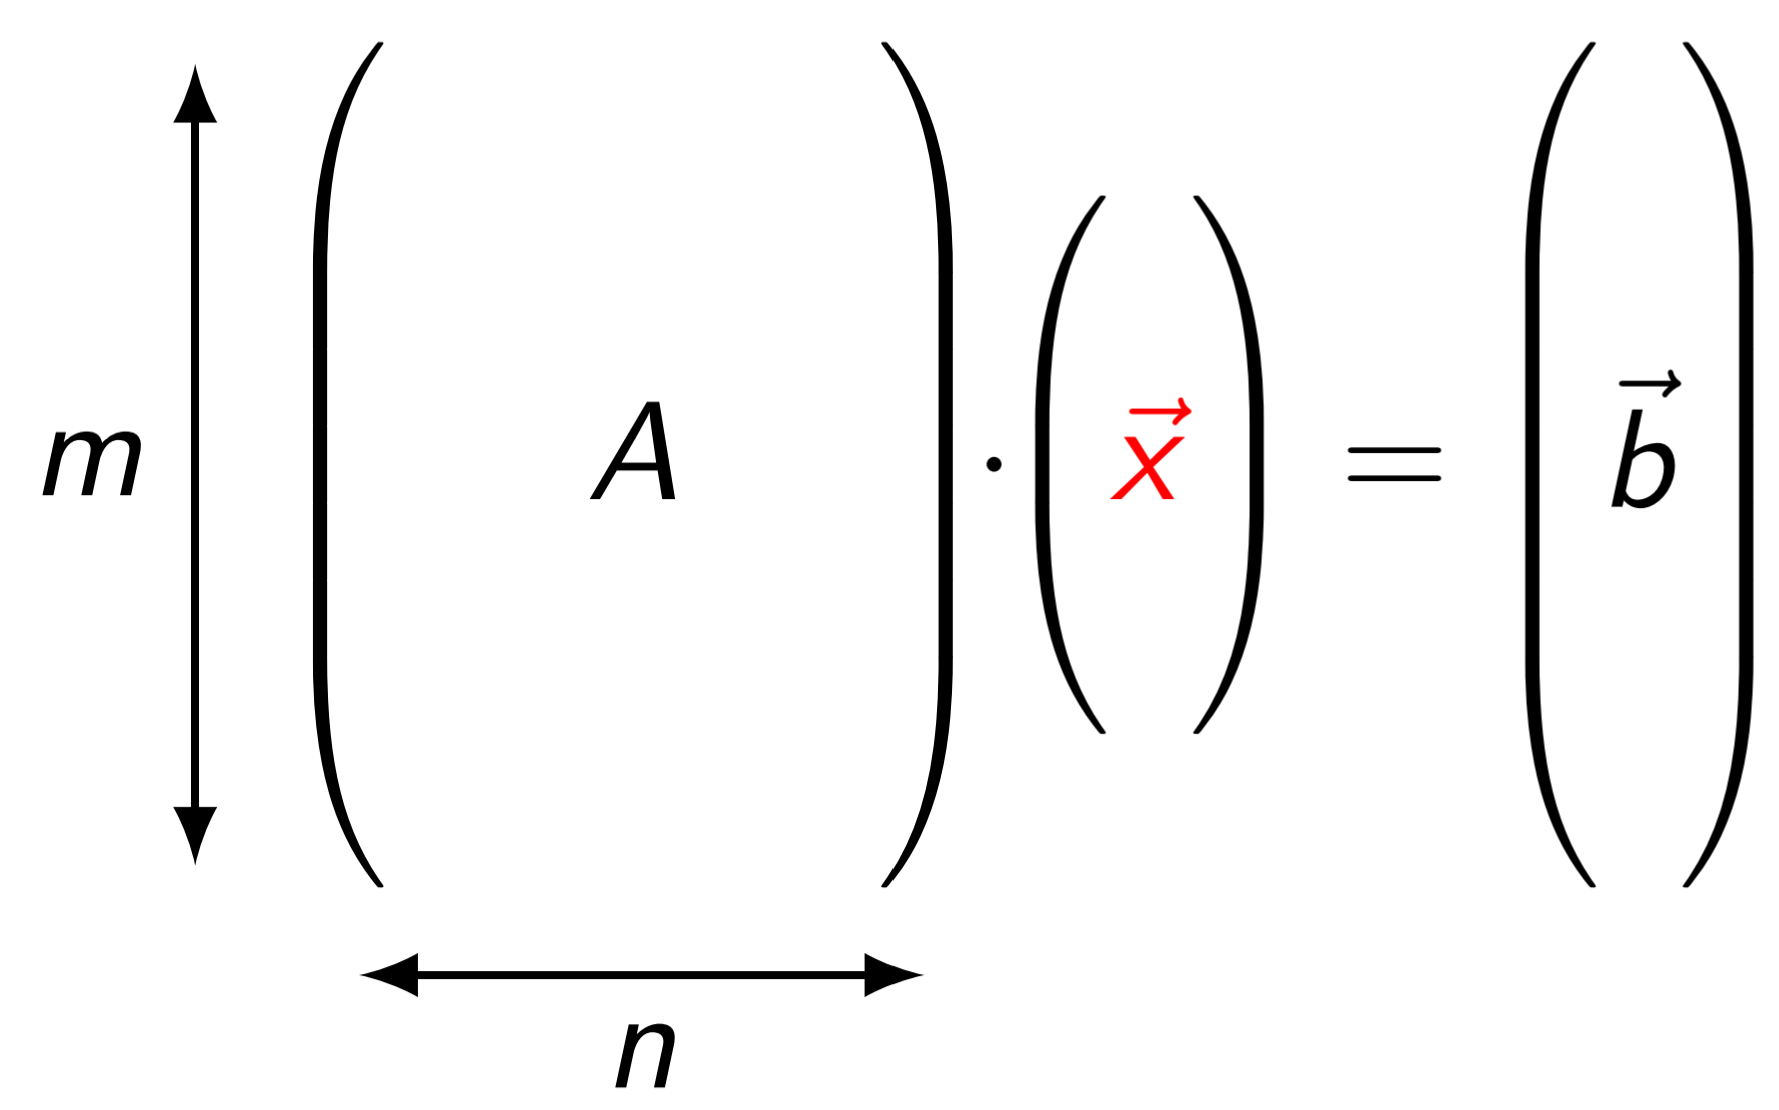
\includegraphics[width=4.5cm]{./bilder/LeastSquare.png}\\
		
		$\boxed{A^{t} A \vec{x}=A^{t} \vec{b} \quad \Rightarrow \quad \vec{x}=\left(A^{t} A\right)^{-1} A^{t} \vec{b}}$
	\end{minipage}\qquad \vline \quad%
	\begin{minipage}[b]{0.3\textwidth}
		\textbf{Inverse}\\[2mm]
		$A^{-1}=\dfrac{1}{\operatorname{det}(A)} \cdot a d j(A) \quad$\\[2mm]
		Sofern $\operatorname{det}(A) \neq 0,$ A regulär\\[5mm]
		$\boxed{A^{-1}=\dfrac{1}{a d-b c} \cdot\left[\begin{array}{cc}{d} & {-b} \\ {-c} & {a}\end{array}\right]}$\\
	\end{minipage}\qquad%
	\begin{minipage}[b]{0.35\textwidth}
		\textbf{Transponierte}\\[2mm]
		\begin{minipage}{0.5\textwidth}			
			Zeilen und Spalten werden vertauscht.
		\end{minipage}%
		\begin{minipage}{0.5\textwidth}
			\quad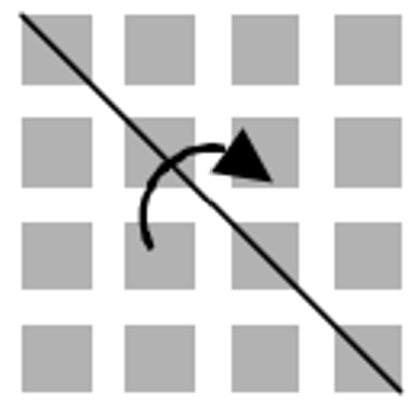
\includegraphics[height=1cm]{./bilder/Transponierte.png}
		\end{minipage}\\[5mm]
		
		$A = \left[\begin{matrix} a_1 \\ a_2 \end{matrix}\right] \quad \Rightarrow \quad A^T = \left[\begin{matrix} a_1 & a_2 \end{matrix}\right] $
	\end{minipage}